%%%%%%%%%%%%%%%%%%%%%%%%%%%%%%%%%%%%%%%%%%%%%%%%%%%%%%%%%%%%%%%%%%%%
\section{\sysname design}\label{sec-design}
%%%%%%%%%%%%%%%%%%%%%%%%%%%%%%%%%%%%%%%%%%%%%%%%%%%%%%%%%%%%%%%%%%%%

 \sysname has
seven components (see Figure~\ref{fig-components}). We first overview
these components and then, in Section~\ref{sec-uses}, describe two
typical testbed scenarios: an experimenter running an experiment, and
a new device joining the testbed. Then, in Section~\ref{sec-interface}
we describe the key set of interfaces.

\subsection{\sysname components}
The components in \sysname have three possible locations: the device
host system (where an experiment runs), the testbed provider (that
organizes and keeps track of testbed resources), and the
experimenter's local host (where experiments are initiated).

%%%%%%%%%%%
%\subsection{\sysname components}
%\label{sec-component}
%%%%%%%%%%%


%%%%%%%%%%%
\paragraph{\fontsize{11.6}{14}\selectfont Device host system.}
Devices provide resources for experimenters to use in their
experiments.
%
To isolate experimenter code from the device host system,
experimenters' code executes in a \textbf{sandbox} component. The default
sandbox in \sysname is a Python-based sandbox~\cite{RepySandbox} that uses language-based
isolation to mitigate the impact of bugs in experimenter
code. The \textbf{resource manager} listens for remote commands 
and mediates access to the sandboxes on a
device, such as authenticates access, starts and stops sandboxes, etc.
%
%%  It providers to remotely
%% access and control the sandboxes on a device.
%% The details about how the
%% resource manager controls the sandbox is presented in
%%Section~\ref{sec-interface}.
%
%Finally, the \textbf{device manager} handles installation and
%software updates of the sandbox and the resource manager.  During
%installation the device manager optionally benchmarks the device
%resources. Once installed, it periodically checks in with the testbed
%provider and re-installs the local components when there are software
%updates.


\begin{table}%[t]
\scriptsize
\centering
%\begin{tabular}{|l|>{\centering\arraybackslash}m{1.8cm}|>{\centering\arraybackslash}m{1.8cm}|}
\begin{tabular}{|p{.23\columnwidth}|p{.44\columnwidth}|p{.18\columnwidth}|}
%\begin{tabular}{|l|l|l|}
\hline

\textbf{Component} & \textbf{Function} & \textbf{Location} \\ \hline

Sandbox & Isolates experimenter code. & \multirow{2}{.18\columnwidth}{Device host system} \\ \cline{1-2}

Resource manager & Mediates access to sandboxes. & \\ \hline

%Device manager & Installation and software updates. & \\ \hline
 
\multirow{2}{*}{Clearinghouse} & Tracks experimenters, mediates experimenter access to devices. & \multirow{3}{.18\columnwidth}{Testbed provider} \\ \cline{1-2}

%Install builder & Builds custom installers. &  \\ \cline{1-2}

Lookup service & Device discovery. & \\ \hline
 
Experiment management tool & Helps experimenters to deploy and run experiments. 
& Experimenter's local host \\ \hline

\end{tabular}
\caption{\small \sysname components, and their function and location.}
\label{tab:components}
%\vspace*{-15pt}
\end{table}

%%%%%%%%%%%%%%%%%%%%%%%%%%%%%%%%%%%%%%%%%%%%%%
\begin{figure}
\center{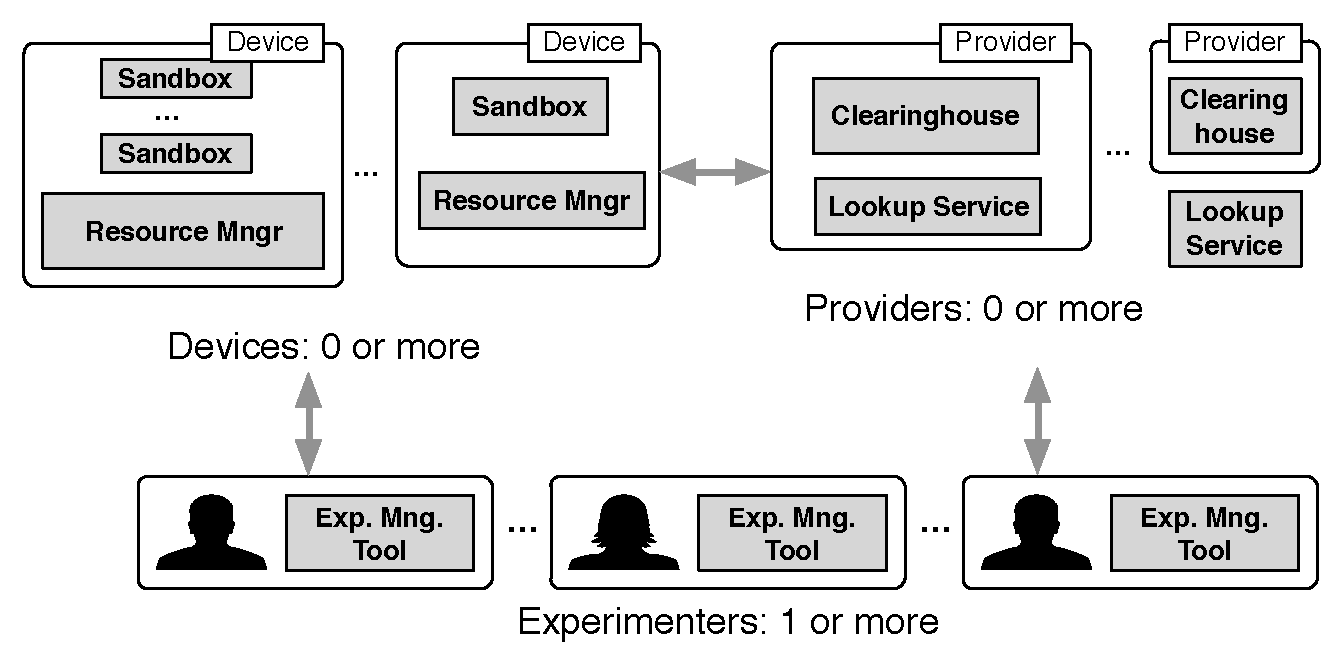
\includegraphics[width=\columnwidth]{figures/arch.pdf}}
\vspace*{-20pt}
\caption{\small \sysname architecture and different components. 
\label{fig-components}\vspace*{-10pt}}
\end{figure}
%%%%%%%%%%%%%%%%%%%%%%%%%%%%%%%%%%%%%%%%%%%%%%



%%%%%%%%%%%
\paragraph{\fontsize{11.6}{14}\selectfont Testbed provider.}
The testbed provider helps experimenters to acquire and manage testbed
resources. 
%and may implement policies to incentivize participation in the testbed.
%
A \textbf{clearinghouse} keeps track of experimenters and mediates
experimenter access to the available sandboxes. Its key role is to
facilitate device sharing, which relieves individual experimenters
from recruiting devices to join their testbeds. The
clearinghouse also allows device owners to download the \sysname
software to add new devices to the testbed.
%
%To join \sysname, a device owner first accesses an \textbf{install
%  builder} and downloads an installer for his host system. The device
%manager, resource manager, sandbox, and a set of public keys are
%packaged into this installer by the install builder. 
After an installation, the resource manager on the device uses the public keys
to register the device in a \textbf{lookup service} so that the device
can be later discovered by experimenters and other testbed components.
%
%Although in this paper we associate the install builder and
%lookup service with the testbed provider, in practice, these two
%components do not need to be under a provider's control.
%%
%Furthermore, the Tsumiki model can support multiple providers that mediate
%access to the same set of devices. That is, a device may simultaneously
%participate in more than one testbed.

%%%%%%%%%%%
\paragraph{\fontsize{11.6}{14}\selectfont Experimenter's local host.}
Experimenters use their local machines to initiate and control
experiments on \sysname.
%
The \textbf{experiment management tool} (EMT) allows experimenters to
deploy and run experiments in sandboxes on remote devices they
requested through the clearinghouse. The EMT first looks up the set of
sandboxes associated with an experimenter in the lookup service, and
caches this list. It then communicates directly with the resource
manager running on these devices, executing commands on behalf of the
experimenter.
%There are variations of EMTs that service different user 
%bases and serve different roles.

All the components above, their functions and locations are listed in 
Table~\ref{tab:components}.

%%%%%%%%%%%%%%%%%%%%%%%%%%%%%%%%%%%%%%%%%%%%%%
\subsection{Overview through testbed scenarios}
\label{sec-uses}
%%%%%%%%%%%%%%%%%%%%%%%%%%%%%%%%%%%%%%%%%%%%%%

We now walk through two testbed scenarios to show how different
components in \sysname interact. We first describe the scenario in
which Bob, an experimenter, runs his experiment on \sysname. 
Then, we describe a scenario in which Alice, a device owner,
contributes her device to the testbed.

%
%% ivan: we can move some of this text into scenario 2 intro, but it
%% doesn't belong here (it's too detailed/early).
%
%% User keys, though not a component, play a critical role. First,
%% they are used to authenticate an experimenter to do an
%% experiment. Second, they are also used to \textit{advertise} device
%% availability. Each device uses a unique user key to place their
%% current \texttt{IP:port} in a DHT, so other parties that know this
%% key can look it up and get information to communicate with this
%% device: this is user keys' third role, where they are used to
%% \textit{discover} resources. Note that there is a special case
%% where user keys are used for advertise-discover, where a key is not
%% to represent a single experimenter, but to represent the
%% clearinghouse.  We will show an example in Scenario 2.
%%
% A set of devices advertise their availability using this user key to
% indicate their intention to join the testbed.


%%%%%%%%%%%%%%%%%%%%%%%%%
\paragraph{Scenario 1: Bob runs an experiment.}
%%%%%%%%%%%%%%%%%%%%%%%%%

\emph{Experimenter registers an experiment with the testbed.} 
When Bob, a wireless researcher, registers an experiment account 
through the \sysname clearinghouse, he first needs to obtain an IRB 
approval for his experiment from his instituion. Then Bob will give 
a detailed description of his experiment according to his IRB approval 
to our clearinghouse, 
including the types of sensors needed (cellular and GPS), 
and the accuracy necessary to carry out the experiment (described 
below). The \sysname clearinghouse then creates 
a set of data filtering policies to ensure that only the specified 
sensors can be accessed by Bob, with the precision 
as specified in Bob's experiment description. For example, Bob's 
experiment can \textit{only} access (1) cellular signal strength, and (2) 
GPS locations at the granularity of zipcode-identified zones in a city. 
Bob also provides a public/private key pair that is unique to Bob.

\emph{Experimenter requests resources on a testbed device.} 
After registration, Bob then requests a sandbox. The clearinghouse first 
uses the lookup service to lookup the available sandboxes. These 
sandboxes advertise themselves using a key that is unique to the testbed. 
After finding a suitable sandbox,
%which satisfies the clearinghouse policy and Bob's constraints (e.g.,
%only sandboxes on devices in North America), 
the clearinghouse contacts the resource manager running on the device. 
%associated with the sandbox. 
The clearinghouse instructs the resource manager to
change the user of the sandbox on the device to Bob, which will set 
the user key for this sandbox to Bob's public key. The resource manager then 
%on the device then
%advertises this sandbox to Bob. It does this through the lookup
%service, 
appends the IP and port of the sandbox to the current value of Bob's
public key in the lookup service. This allows Bob to look up
the sandbox that he requested.

Meanwhile, the requested sandbox receives the policies associated with 
Bob's experiment from the clearinghouse. The sandbox then implements specific 
filtering rules for each policy. For policy (1) above, the sandbox 
imposes a restriction that only cellular signal strength (no cell tower 
IDs, cellular technologies, etc.) can be accessed; for policy (2), 
the sandbox blurs the GPS location returned from the device 
down to the coordinates of zipcode regions. 

%%%%%%%%%%%%%%%%%%%%%%%%%%%%%%%%%%%%%%%%%%%%%%
\begin{figure}
\center{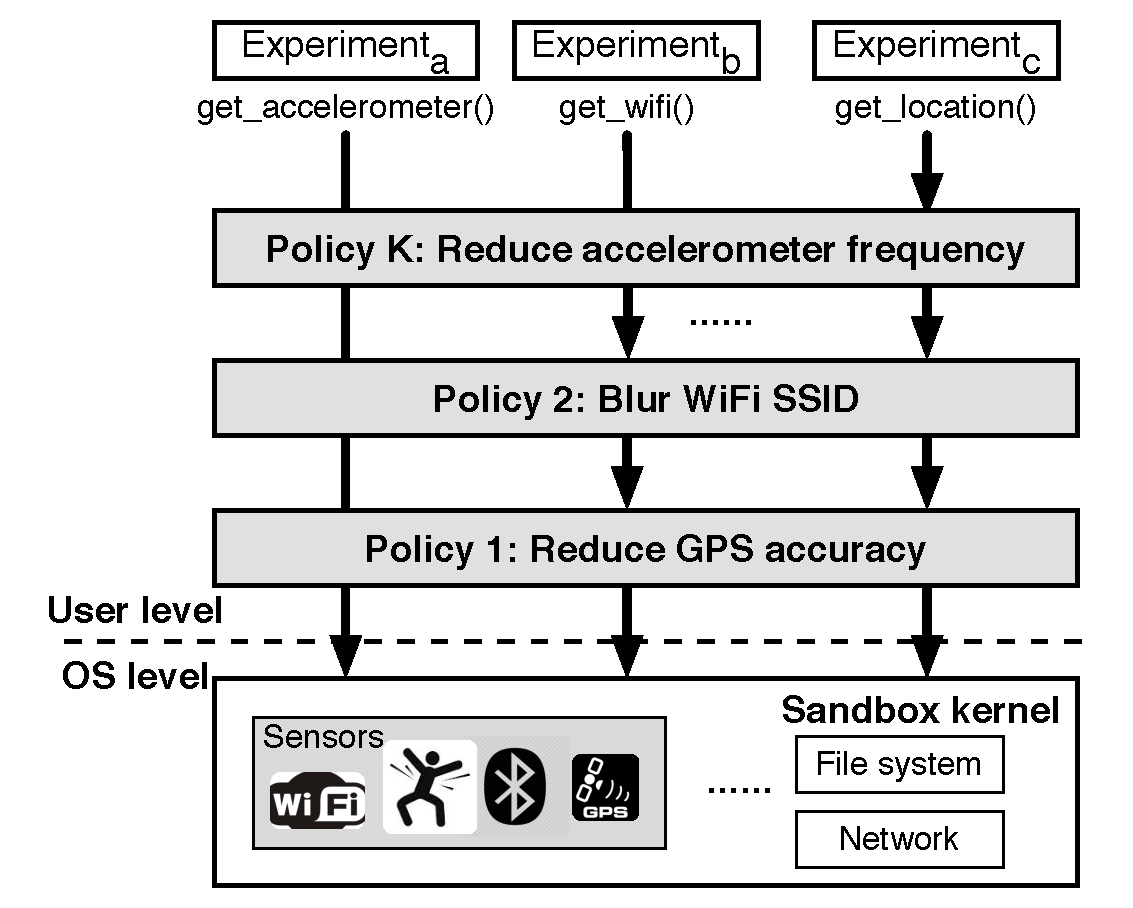
\includegraphics[width=.38\textwidth]{figures/blur.pdf}}
%\vspace*{-20pt}
\caption{\small \sysname blur policies. 
\label{fig-blur}}
\end{figure}
%%%%%%%%%%%%%%%%%%%%%%%%%%%%%%%%%%%%%%%%%%%%%%


\emph{Experimenter runs code in a device sandbox.} Next, Bob uses the
experiment management tool (EMT) to control the acquired sandbox from
his local machine. The default EMT is a shell through which
experimenters execute commands.
%
Bob first loads his public and private keys into the EMT. The EMT uses Bob's
public key to look up the previously acquired sandbox in the lookup
service. This returns the
\texttt{IP:port} of the resource manager on the device. %with Bob's sandbox
Bob can now make calls to the resource manager (through EMT
commands) to control his sandbox. 

Bob's experiment code is written in Python-like language, which provides
calls to the file system, network interface, sensors, etc. on the device. The
code in Bob's experiment is subject to the policies set up during his 
experiment registration stage. As shown in Figure~\ref{fig-blur}, if Bob's 
experiment code calls \texttt{get\_location()} and Bob's IRB policy restricts
that the location coordinates returned from the device be blurred down to 
the coordinates of zipcode regions, then the result of \texttt{get\_location()}
will be reduced to the granularity of a zipcode region. Similarly, WiFi SSID
can be blurred to a hashed string for privacy reasons, the frequency to 
access an accelerometer can be restricted to prevent inferring passwords 
from the movement and tilt of the device. If Bob's IRB disallows Bluetooth
measurement, then the access to the Bluetooth interface can be entirely 
blocked by the policy.

%To run his {\tt helloworld} program
%Bob issues the \texttt{run helloworld} command, which instructs the
%remote resource managers to upload the file \texttt{helloworld} from
%Bob's local host to the sandbox (by calling
%\texttt{AddFileToSandbox()}), and then start executing this program
%(by calling \texttt{StartSandbox()}). Bob can then check the state of
%his sandbox with the EMT \texttt{list} command, and look through the
%console log output of the {\tt helloworld} program with the
%\texttt{show log} command. A set of common EMT commands and the associated
%(remote) resource manager calls are listed in Table~\ref{tab:emt-rm-calls}.
%\todo{Albert: Shall we list the API calls for list and show log, too?}

% (as one of the states in Figure~\ref{fig-sandboxstatus})

\emph{Experimenter releases the acquired resources.}  When Bob is done
with his experiment, he may release his sandbox explicitly
through the clearinghouse. To prevent experimenters from holding onto unused resources,
the clearinghouse may also implement a policy 
to expire acquired sandboxes after a
timeout (i.e., resources must be periodically renewed to prevent
expiration).
%Note that expiration is a testbed-specific policy, implemented 
%at the clearinghouse (Section~\ref{sec-policy}).
%\ivan{Expiration seems like a policy; implemented at CH; mention this.} 
In both cases the clearinghouse will instruct the resource manager on device to
remove Bob's public key from the sandbox, and reset the sandbox (e.g., delete 
all experiment code uploaded by Bob).


%%%%%%%%%%%%%%%%%%%%%%%%%%%%%%%%%%%%%%%%%%%%%%%%%%%%%%%%%%%%%%%%
%\begin{table}%[t]
%\scriptsize
%\centering
%\begin{tabular}{|l|l|} \hline
%\textbf{EMT command} & \textbf{Corresponding resource manager calls} \\\hline
%
%\multirow{2}{*}{\texttt{run program-name [args]}} & \texttt{AddFileToSandbox(program-name, ..)} \\ 
%& \texttt{StartSandbox(program-name, args, ..)} \\ \hline
%
%\texttt{stop} & \texttt{StopSandbox()} \\ \hline
%
%\texttt{list} & \texttt{GetSandboxStatus()} \\ \hline
%
%\texttt{show log} & \texttt{ReadSandboxLog()}\\ \hline
%
%\texttt{download filename} & \texttt{RetrieveFileFromSandbox(filename, ..)} \\ \hline
%
%\texttt{upload filename} & \texttt{AddFileToSandbox(filename, ..)} \\ \hline
%
%\texttt{show files} & \texttt{ListFilesInSandbox()} \\ \hline
%
%%\end{tabular}
%
%%\begin{tabular}{|l|l|} \hline
%
%\hline\hline
%
%\multirow{2}{*}{\texttt{browse}} & Lookup service:\texttt{~~~Get(user-pubkey)} \\ 
%& Resource manager:\texttt{~GetSandboxStatus()} \\ \hline
%
%\end{tabular}
%
%\caption{\small Commands for the default experiment management tool in
%  Tsumiki and the corresponding resource manager calls; {\tt browse}
%  is an exception (it makes calls to both the lookup service and the
%  resource manager). The EMT commands are issued by an experimenter from
%  his local host.}
%\label{tab:emt-rm-calls}
%\vspace*{-15pt}
%\end{table}
%%%%%%%%%%%%%%%%%%%%%%%%%%%%%%%%%%%%%%%%%%%%%%%%%%%%%%%%%%%%%%%%

%% The scenario above extends to multiple sandboxes.

%%%%%%%%%%%%%%%%%%%%%%%%%
\paragraph{Scenario 2: Alice contributes a device to the testbed.}  
%%%%%%%%%%%%%%%%%%%%%%%%%

%% In this scenario Alice installs software from a Tsumiki testbed to 
%% allow the resources on her device to be used.  Much like the previous
%% scenario, the clearinhhouse will locate Alice's install using a sandbox user 
%% key.

%In this scenario we re-use the sandbox user key. However, when Alice
%installs testbed software on her device, the sandboxes on her device
%will use a public key owned by a clearinghouse, not Alice, or another
%experimenter. Alice's device will advertise itself with this key to
%indicate its intent to join the testbed.

%%  To add or remove a user key, the same
%% \texttt{ChangeUsers()} is called on all the resource managers having
%% this user key.

\emph{Device installation.} When Alice, a device owner, decides to
contribute her device to a testbed, she first downloads a
testbed-specific installer through the clearinghouse. The
clearinghouse creates this installer with a key, \texttt{node-join-key}, 
that is unique to the testbed and is used by new devices to advertise 
themselves through the lookup service. 
%The install builder packages this key with the device manager, resource
%manager, and sandbox into a set of platform-specific installers.
%%
During installation, the device manager benchmarks the device system,
and saves the result to use for later configuration.
%%  in data structure
%% \texttt{benchmark-results} (see Table~\ref{tab:datastructs}).
%%
%\ivan{%build-installer should take an advertise key as an arg, no? 
%What is ip:port of lookup-service, is that another arg to the
%  build-installer, or is this hard-coded in the CIB?}

%%  by calling
%% \texttt{build-installers()}. %\ivan{benchmarking?  split/merge?}

\emph{Device discovery.} There are three steps to discovering Alice's
new device. (1) When the resource manager on Alice's device starts, it 
advertises its \texttt{IP:port} of the sandboxes to the lookup service by 
calling \texttt{Put(node-join-key, IP:port)}. The clearinghouse periodically
calls \texttt{Get(node-join-key)} on the lookup service to discover
new devices installed with the testbed-specific installer. (2) After
discovering Alice's device, the clearinghouse contacts the resource
manager on her device, instructs the resource manager to
configure the sandboxes according to the benchmark results, and
instructs the sandbox to implement different data policies.
%
%%  split
%% or join the sandboxes by \texttt{SplitSandbox()} or
%% \texttt{JoinSandboxes()} call according to \texttt{benchmark-results}
%% and clearinghouse policy (details about policy in
%% .
%%
%% Next, \texttt{node-join-key} is copied into the new sandboxes.
%%
%%  The
%% resulting sandbox sizes and key information is kept in a data
%% structure \texttt{sandboxinfo}.
%% \yanyan{Please check if this is
%%  correct.}
(3) The clearinghouse asks the resource manager to change the
\texttt{\texttt{node-join-key}} on Alice's device to the \texttt{node-ready-key}. 
The resource manager will then advertise its
\texttt{IP:port} using this new key and the clearinghouse will record
that Alice's device successfully joined the testbed.

